Mobile devices have become a huge part of our lives, offering an extensive set of functionalities such as internet access, banking, high quality camera and microphones, global location services, and much more. The Android platform is the most used mobile platform in the world, with 71.63\% market share and 3.6 billion users worldwide \cite{turner_how_nodate}. Android applications, commonly known as \textit{apps}, are distributed in various marketplaces, with Google Play Store being the largest and most used having over 3.5 million apps available \cite{turner_how_nodate-1}. The huge popularity of mobile devices combined with the access to many sensitive capabilities have turned mobile devices on attractive targets for malicious actors. In fact, Truong et al. have reported that over 0.25\% of Android devices were infected with malware~\cite{truong_company_2014}.

% falar sobre repackaging class, citar MAS pra resolver esses caras
Most Android malware employ a type of attack called \textit{repackaging}, which consists of altering an existing application to introduce malicious behavior. These repackaged apps are distributed in various marketplaces, and trick users into believing that they're downloading the original version of the app. Once installed on a device, these harmful applications are capable of capturing user input, recording data from the microphone or camera and sending it to third-party servers.

To address this issue, previous works studied a method called \textit{mining sandboxes}, first proposed by Jamrozik et al.~\cite{jamrozik_mining_2016} that consists on capturing an app behavior using automated test generation tools. Bao et al. demonstrated that mining sandboxes are an effective mechanism to detect malicious activity on Android apps, and also compared which test case generation tools produced the best results for this purpose \cite{bao_mining_2018}. Building up on Bao et al's study, Costa et al.~\cite{costa_exploring_2022} developed a tool called DroidXP that combines static analysis with the dynamic analysis proposed by the mining sandboxes approach to achieve a higher effectiveness on malware detection. Le et al.~\cite{le_towards_2018} have also extended Jamrozik's work by creating a more robust sandbox that not only considers new behaviors introduced by repackaged versions of the apps, but also identifies differences on existing behaviors, such as different arguments passed to sensitive methods.

In this study, we aim to develop the existing technique by conducting a more comprehensive study, where we will evaluate the performance of combining Costa's approach of considering a static analysis along with the dynamic analysis \cite{costa_exploring_2022}, with Le's proposal of comparing arguments passed into sensitive APIs \cite{le_towards_2018} to detect Android repackaged malware. In addition, previous studies have utilized small datasets, with 102 pairs of apps for~\cite{bao_mining_2018} and~\cite{costa_exploring_2022}, and 25 pairs for~\cite{le_towards_2018}, which may compromise the external validity of the findings. To address this issue, we will use a significantly larger dataset consisting of 1,707 pairs. In general, to achieve the goals of this study, we adapted the  DroidXP framework~\cite{costa_droidxp_2020}, so that it could be able to instrument Android apps and capture the arguments passed to a given set of methods.

% falar da avaliacao, falar como performou, e como a familia influencia
The primary contribution of this work lies on the evolution of the DroidXP framework and the evaluation of this new approach regarding the accuracy of its malware detection capabilities. Our results indicate that there is a slight improvement of 3.51\% on the overall accuracy if compared to the previous version, and the detection capabilities of this new approach are highly dependant on the malware family. While some families show a substantial improvement in detection rates, others express no relevant change.

\begin{figure}
    \centering
    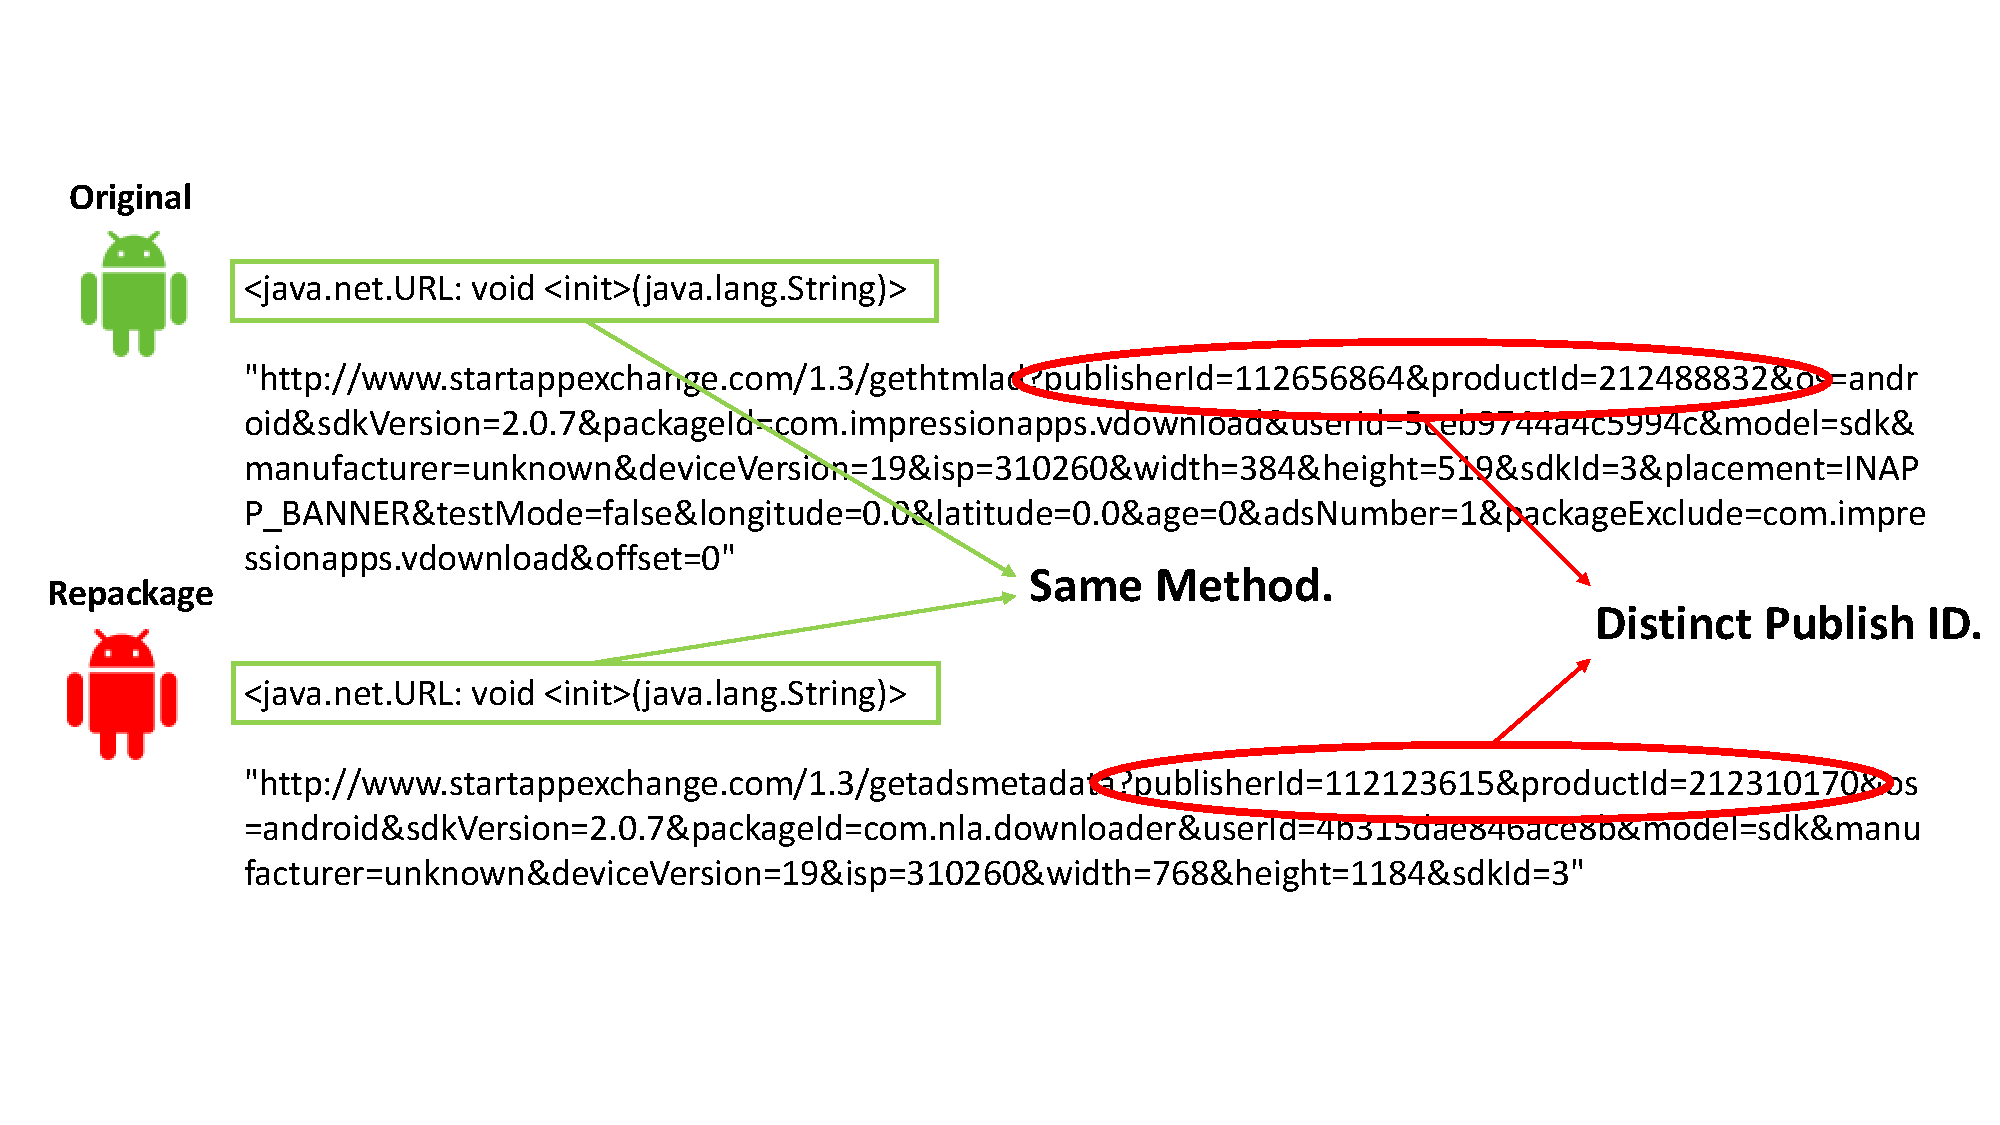
\includegraphics[width=0.8\textwidth]{img/parameterDiff.pdf}
    \caption{Example of a successful detection comparing the arguments passed to sensitive methods. In this example, the internet connection API is used to access a advertisement URL. The advertisement URL is changed to redirect ad revenue to the publisher of the repackaged version of the app.}
    \label{fig:successful-detection-example}
\end{figure}

% falar da estrutura do doc????